\chapter{Beheer, Validatie en Verificatie}
In dit hoofdstuk wordt beschreven hoe de kwaliteit van het eindproduct is bewaard.
Eerst wordt behandeld de afstudeer voortgang gesprekken zijn gedaan samen met de codereviews.
Daar na wordt de Versiebeheer en Codestandaarden inbeeldt gebracht.
Vervolgens  wordt het proces en de bewaking daarvan besproken
En als laatste wordt het testrapport besproken
% \input{Content/4_Beheer-Validatie-Verificatie/Procesbewaking.tex}
% \section{Originele eisen en wensen}
In deze sectie wordt er besproken welke requirements niet mee genomen zijn voor het eind resultaat.
In sectie \ref{section:Eindproduct} wordt het gerealiseerde eindproduct besproken.
Er is besloten om 2 requirements niet te realiseren voor het eindproduct.
Deze requirements zijn: 

\whitespace
\textbf{KB-FR6, Authenticatie en identificeren}

\whitespace
Het authenticeren en identificeren van de \gls{Beheerder} is een requirement wat besloten is om te laten vallen voor het proof of concept.
De requirement was origineel verkeerd ingeschat aan hoeveel waarde het zou opleveren aan het project.
Samen met de product owner is er toen besloten om de realisatie van deze requirement een lagere prioriteit te geven.
Helaas was er geen tijd over om deze functionaliteit te implementeren.

\whitespace
\textbf{KB-FR10, Formulieren}

\whitespace
Formulieren zijn een belangrijk onderdeel voor verschillende webapplicaties.
Verder is het een belangrijk deel van het huidige \gls{CMS}.
Tijdens het ontwerpen van het datamodel kwam al naar voren dat formulieren implementeren veel werk zou kosten.
Hierom is er besloten dat formulieren niet tijdens de afstudeerperiode te realiseren.

% \newpage
%
\section{Codereviews en Afstudeerstage voortgang}
\label{section:CodereviewsEnStageVoortgang}
Tijdens de afstudeer periode is er een keer per week een gesprek ingepland met de afstudeer begeleider Thom Koenders (senior software engineer).
Deze gesprekken gingen over de huidige stand van zaken en wat de moglijke problemen die er waren.
Verder is het ook vaak over de opzet van de architectuur en de code gegaan.

\whitespace
Verder werden er ook codereviews gebruikt voor dat de code gemerged werdt op de main branch.
Dit werdt gedaan door de verschillende specialisten in hun vak.
Voor de backend code is Kevin Sneider (backend software enigneer) benaderd voor deze reviews.
En voor de frontend is Maks Tennebroek (frontend software engineer) benaderd.

\section{Versiebeheer}
Voor versiebeheer is er gebruik gemaakt van git en als repository platform Bitbucket.


\section{Codestandaarden}
Tijdens het ontwikkelen van de afstudeeropdracht is er gecontrolleerd op de code standaarden die gebruikt zijn.
Deze controlles werden tijden de code reviews en stagevoortgang besproken (Zie sectie \ref{section:CodereviewsEnStageVoortgang}).
% Omdat Snakeware niet een vaste guideline heeft voor code standaarden is er zelf een opgesteld die gevolgt is tijdens de afstudeeropdracht.
% Deze standaarden staan vermeld in de bijlage \textbf{(bron)}.

\section{Process en bewaking}
Tijdens de afstudeerperiode is er gewerkt met een Agile \parencite{Agile} methode genaamd Scrum \Parencite{Scrum}.
Er is gewerkt met sprints van 2 weken waar bij de requirements opgedeeld werden in kleine stukjes.
Dit is gedaan om de taken behapbaar te maken en om snel veranderingen te kunnen aanbrengen.
Elke week werd er met de afstudeerbegeleider de progressie gesproken van de week waar bij mogelijk bijgestuurd werd.
De verschillende sprints werden bijgehouden in een notitie programma \textbf{Obsidian} hierbij is elke sprint opgedeeld in een apparte note.
Vervolgens is er gebruikgemaakt van een scrumboard om de progressie bij te houden dit werd ook gedaan in Obsidian.
In figuur \ref{fig:VoorbeeldSprint} is te zien hoe zo'n sprint ingepland werdt.

\whitespace[2]
\begin{graphic}
	\captionsetup{type=figure}
	\caption{Sprint 4 van het realisatie process}
	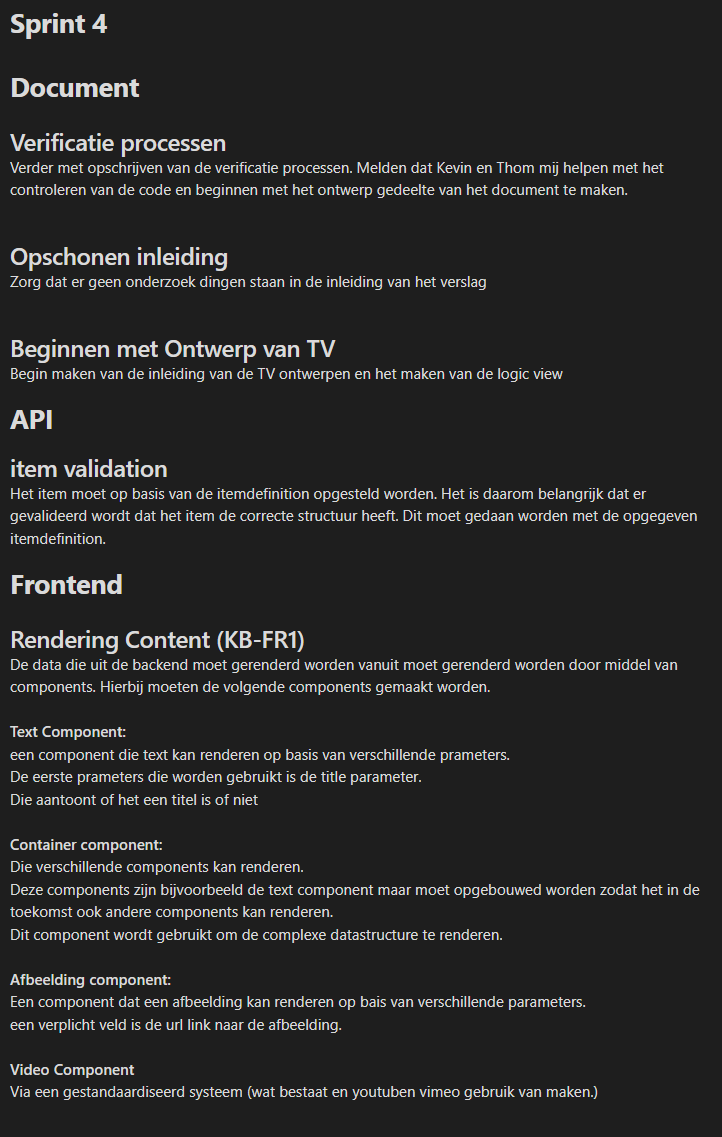
\includegraphics[scale=0.5]{SprintVoorbeeld.png}
	\label{fig:VoorbeeldSprint}
\end{graphic}


\newpage
\section{Testrapport}
Tijdens het ontwikkelen van het eindproduct zijn er verschillende testen uitgevoerd.
Er is gebruik gemaakt van het V-model de Teststrategie die gebruikt wordt is beschreven in sectie \ref{section:Teststrategie}.
In dit hoofdstuk worden de verschillende testen toegelicht en behandeld.

\subsection{Unittesten}
Voor het unit testen van de API is er gebruikgemaakt van xUnit (voor meer informatie zie sectie \ref{section:Bouwomgeving}).
Unit testen worden gebruikt om de verschillende logica van het systeem te testen.
Hierom zijn testen geschreven voor de handlers en de data mappers in de applicatie.
Een voorbeeld van zo'n unit test is te zien in figuur \ref{fig:ExampleUnitTest}.
Verder is er een overzicht van de verschillende unittesten in figuur \ref{fig:OverviewUnitTests}.

\whitespace[2]
\begin{graphic}
	\captionsetup{type=figure}
	\caption{Geïmplementeerde unit test}
	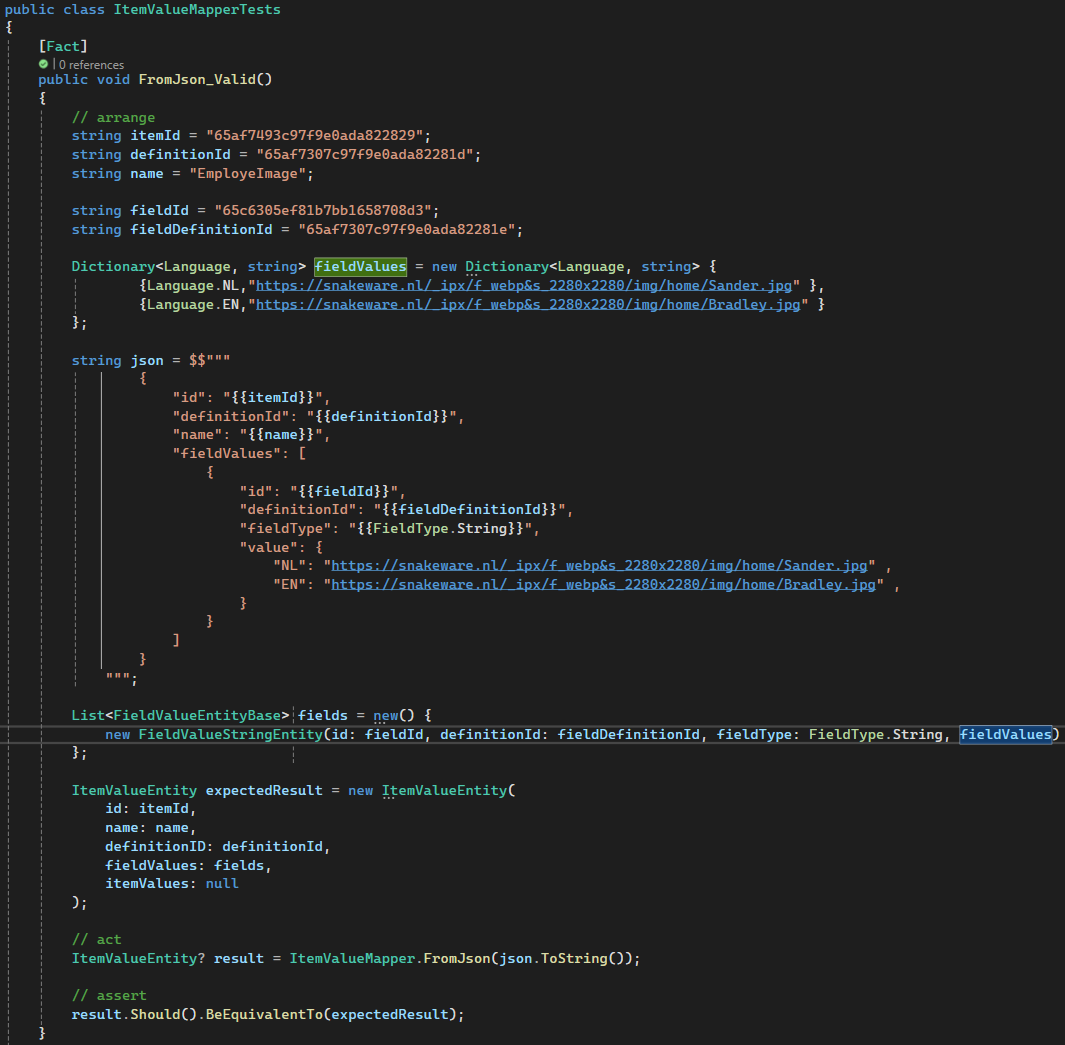
\includegraphics[scale=0.52]{ExampleUnitTest.png}
	\label{fig:ExampleUnitTest}
\end{graphic}

\subsection{Intergratietesten}

\subsection{Systeemtesten}
Voor de systeemtesten zijn de webapplicatie en API handmatig getest.
Tijdens deze testen werd er gekeken of alle functionele en niet-functionele requirements van de applicatie werkte.
Hierbij wordt er gecontroleerd of de nieuwe functionaliteit voldoet aan de vastgesteld applicatiecriteria.

\whitespace
Als een functionaliteit klaar was werd deze apart nog een keer getest.
Eerst werd de API getest via swagger en daarna werd er gekeken of de functionaliteit ook goed werkte op de frontend.

\subsection{Acceptatietesten}
Een van de randvoorwaarden was dat er geen \gls{GUI} wordt gemaakt voor het beheer van het CMS.
Dit is gedaan om de scope van de opdracht reëel te houden en binnen de afstudeerperiode.
Het nadeel hiervan is dat het lastig is om acceptatie uit te voeren is die betrekkingen hebben tot de \gls{Beheerder}.
Daarom is er besloten om geen acceptatie testen uit te voeren.


\section{Originele eisen en wensen}
In deze sectie wordt er besproken welke requirements niet mee genomen zijn voor het eind resultaat.
In sectie \ref{section:Eindproduct} wordt het gerealiseerde eindproduct besproken.
Er is besloten om 2 requirements niet te realiseren voor het eindproduct.
Deze requirements zijn: 

\whitespace
\textbf{KB-FR6, Authenticatie en identificeren}

\whitespace
Het authenticeren en identificeren van de \gls{Beheerder} is een requirement wat besloten is om te laten vallen voor het proof of concept.
De requirement was origineel verkeerd ingeschat aan hoeveel waarde het zou opleveren aan het project.
Samen met de product owner is er toen besloten om de realisatie van deze requirement een lagere prioriteit te geven.
Helaas was er geen tijd over om deze functionaliteit te implementeren.

\whitespace
\textbf{KB-FR10, Formulieren}

\whitespace
Formulieren zijn een belangrijk onderdeel voor verschillende webapplicaties.
Verder is het een belangrijk deel van het huidige \gls{CMS}.
Tijdens het ontwerpen van het datamodel kwam al naar voren dat formulieren implementeren veel werk zou kosten.
Hierom is er besloten dat formulieren niet tijdens de afstudeerperiode te realiseren.

